% vim: set tw=78 sts=2 sw=2 ts=8 aw et ai:

The Stanford Topic Modeling Toolbox returns its results by specifying for each year a corresponding mixture of topics. By browsing over the topic files, one can notice that only very rarely is a year associated with a topic mixture in which there is no single dominant topic. Thus, I have chosen to consider only the most likely topic for each year.

\begin{figure}
\centering
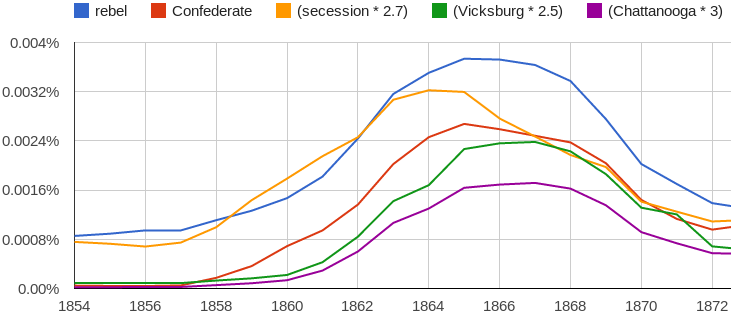
\includegraphics[max size={\textwidth}{\textheight}]{civil-war-related-series}
\caption{Ngram time series related to the American Civil War}
\label{fig:civil-war-related-series}
\end{figure}

Though seemingly the weakest model, the double change algorithm has generated some of the most accurate topics for certain periods of time. For example, the topic for the years $1858$ to $1864$ and $1867$ to $1868$ is composed of the following main words: rebel, confederate, wolff, mcclellan, schleswig, secession, ich, vicksburg, rebels, chattanooga, die, sherman, doge, nicht, wedgwood, holstein, longstreet, gen, flax and der. A lot of these words relate directly to the American Civil War, providing a high degree of confidence that the model has successfully detected this important event in history. A graph comparing the time series of some of the words relating to the American Civil War is shown in \autoref{fig:civil-war-related-series}.

\begin{figure}
\centering
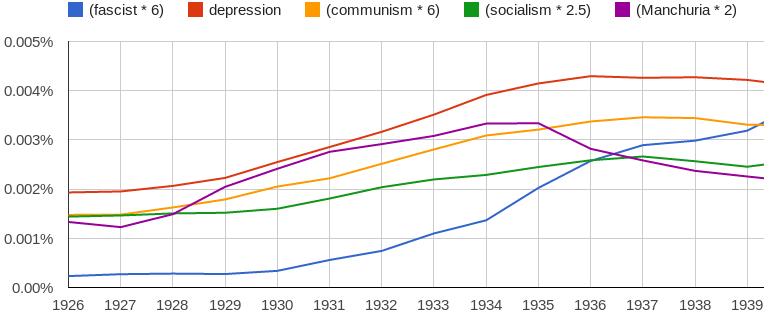
\includegraphics[max size={\textwidth}{\textheight}]{pre-ww2-related-series}
\caption{Ngram time series related to the pre World War II period}
\label{fig:pre-ww2-related-series}
\end{figure}

For the linear model peak detection, I will consider the time period from $1932$ to $1936$, filled with events that foreshadowed World War II. The detected topic consists of fascist, adjustment, federal, depression, rubber, communism, collective, pact, medieval, vitamin, broadcasting, reconstruction, alpha, recovery, radio, employers, socialism, communists, tomorrow and manchuria. Unlike the case of the American Civil War, there is no underlying important event that could cause the topic to converge. Nonetheless, the selected words, the most relevant of which are shown in \autoref{fig:pre-ww2-related-series}, do a good job of painting an accurate image of that period.

\begin{figure}
\centering
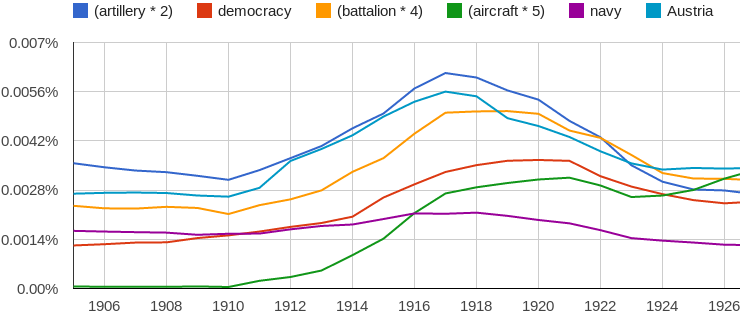
\includegraphics[max size={\textwidth}{\textheight}]{ww1-related-series}
\caption{Ngram time series related to World War I}
\label{fig:ww1-related-series}
\end{figure}

For the last model, Gaussian model peak detection, the interval between $1916$ and $1920$ shall be used, a rough approximation of World War I. Upon training Latent Dirichlet Allocation, the following topic is obtained:artillery, target, syndrome, nationalism, naval, democracy, alcohol, battalion, pan, rehabilitation, defense, dad, von, aircraft, navy, strategic, austria, damping, mobilize and firing. The words pertaining to World War I are shown together in \autoref{fig:ww1-related-series}, scaled such that they are comparable in size.

However, many of the words present in these topics convey little information about a historic event, creating a significant amount of noise. Currently, their removal is done manually, but automating this task will most likely become the target of future research.
